% This is "aamas2012 .tex" August 2012 
% This file should be compiled with "aamas2012 .cls" 
% This example file demonstrates the use of the 'aamas2012 .cls'
% LaTeX2e document class file. It is for those submitting
% articles to AAMAS 2012  conference. This file is based on
% the sig-alternate.tex example file.
% The 'sig-alternate.cls' file of ACM will produce a similar-looking,
% albeit, 'tighter' paper resulting in, invariably, fewer pages.
% than the original style ACM style.
%
% ----------------------------------------------------------------------------------------------------------------
% This .tex file (and associated .cls ) produces:
%       1) The Permission Statement
%       2) The Conference (location) Info information
%       3) The Copyright Line with AAMAS data
%       4) NO page numbers
%
% as against the acm_proc_article-sp.cls file which
% DOES NOT produce 1) thru' 3) above.
%
% Using 'aamas2012 .cls' you don't have control
% from within the source .tex file, over both the CopyrightYear
% (defaulted to 200X) and the IFAAMAS Copyright Data
% (defaulted to X-XXXXX-XX-X/XX/XX).
% These information will be overwritten by fixed AAMAS 2012  information
% in the style files - it is NOT as you are used with ACM style files.
%
% ---------------------------------------------------------------------------------------------------------------
% This .tex source is an example which *does* use
% the .bib file (from which the .bbl file % is produced).
% REMEMBER HOWEVER: After having produced the .bbl file,
% and prior to final submission, you *NEED* to 'insert'
% your .bbl file into your source .tex file so as to provide
% ONE 'self-contained' source file.
%

\newtheorem{note}{Note}
\newtheorem{example}{Example}
\newtheorem{definition}{Definition}

% This is the document class for full camera ready papers and extended abstracts repsectively 

\documentclass{aamas2012}

\usepackage{graphicx}
\usepackage{color}
\usepackage{algorithm,algorithmic}

\graphicspath{{pictures/}}

% if you are using PDF LaTex and you cannot find a way for producing
% letter, the following explicit settings may help
 
\pdfpagewidth=8.5truein
\pdfpageheight=11truein

\begin{document}

% In the original styles from ACM, you would have needed to
% add meta-info here. This is not necessary for AAMAS 2012  as
% the complete copyright information is generated by the cls-files.


\title{Representing Agent reasoning with Meta-Knowledge on ASP Modules Combination}

% AUTHORS


% For initial submission, do not give author names, but the
% tracking number, instead, as the review process is blind.

% You need the command \numberofauthors to handle the 'placement
% and alignment' of the authors beneath the title.
%
% For aesthetic reasons, we recommend 'three authors at a time'
% i.e. three 'name/affiliation blocks' be placed beneath the title.
%
% NOTE: You are NOT restricted in how many 'rows' of
% "name/affiliations" may appear. We just ask that you restrict
% the number of 'columns' to three.
%
% Because of the available 'opening page real-estate'
% we ask you to refrain from putting more than six authors
% (two rows with three columns) beneath the article title.
% More than six makes the first-page appear very cluttered indeed.
%
% Use the \alignauthor commands to handle the names
% and affiliations for an 'aesthetic maximum' of six authors.
% Add names, affiliations, addresses for
% the seventh etc. author(s) as the argument for the
% \additionalauthors command.
% These 'additional authors' will be output/set for you
% without further effort on your part as the last section in
% the body of your article BEFORE References or any Appendices.

%\numberofauthors{8} %  in this sample file, there are a *total*
% of EIGHT authors. SIX appear on the 'first-page' (for formatting
% reasons) and the remaining two appear in the \additionalauthors section.
%

\numberofauthors{3}

\author{
% You can go ahead and credit any number of authors here,
% e.g. one 'row of three' or two rows (consisting of one row of three
% and a second row of one, two or three).
%
% The command \alignauthor (no curly braces needed) should
% precede each author name, affiliation/snail-mail address and
% e-mail address. Additionally, tag each line of
% affiliation/address with \affaddr, and tag the
% e-mail address with \email.
% 1st. author
\alignauthor
Tony Ribeiro\\
       \affaddr{National Institute of Informatics}\\
       \affaddr{Tokyo, Japan}\\
       \email{ribeiro@nii.ac.jp}
% 2nd. author
\alignauthor
Katsumi Inoue\\
       \affaddr{National Institute of Informatics}\\
       \affaddr{Tokyo, Japan}\\
       \email{ki@nii.ac.jp}
% 3rd. author
\alignauthor
Gauvain Bourgne\\
       \affaddr{????}\\
       \affaddr{Paris, France}\\
       \email{bourgne@nii.ac.jp}
}

%\and  % use '\and' if you need 'another row' of author names

% 4th. author
%\alignauthor Lawrence P. Leipuner\\
%       \affaddr{Brookhaven Laboratories}\\
%       \affaddr{Brookhaven National Lab}\\
%       \affaddr{P.O. Box 5000}\\
%       \email{lleipuner@researchlabs.org}

% 5th. author
%\alignauthor Sean Fogarty\\
%       \affaddr{NASA Ames Research Center}\\
%       \affaddr{Moffett Field}\\
%       \affaddr{California 94035}\\
%       \email{fogartys@amesres.org}

% 6th. author
%\alignauthor Charles Palmer\\
%       \affaddr{Palmer Research Laboratories}\\
%      \affaddr{8600 Datapoint Drive}\\
%       \affaddr{San Antonio, Texas 78229}\\
%       \email{cpalmer@prl.com}

%\and

%% 7th. author
%\alignauthor Lawrence P. Leipuner\\
%       \affaddr{Brookhaven Laboratories}\\
%       \affaddr{Brookhaven National Lab}\\
%       \affaddr{P.O. Box 5000}\\
%       \email{lleipuner@researchlabs.org}

%% 8th. author
%\alignauthor Sean Fogarty\\
%       \affaddr{NASA Ames Research Center}\\
%       \affaddr{Moffett Field}\\
%       \affaddr{California 94035}\\
%       \email{fogartys@amesres.org}

%% 9th. author
%\alignauthor Charles Palmer\\
%       \affaddr{Palmer Research Laboratories}\\
%       \affaddr{8600 Datapoint Drive}\\
%       \affaddr{San Antonio, Texas 78229}\\
%       \email{cpalmer@prl.com}

%}

%% There's nothing stopping you putting the seventh, eighth, etc.
%% author on the opening page (as the 'third row') but we ask,
%% for aesthetic reasons that you place these 'additional authors'
%% in the \additional authors block, viz.
%\additionalauthors{Additional authors: John Smith (The Th{\o}rv{\"a}ld Group,
%email: {\texttt{jsmith@affiliation.org}}) and Julius P.~Kumquat
%(The Kumquat Consortium, email: {\texttt{jpkumquat@consortium.net}}).}
%\date{30 July 1999}
%% Just remember to make sure that the TOTAL number of authors
%% is the number that will appear on the first page PLUS the
%% number that will appear in the \additionalauthors section.

\maketitle

\begin{abstract}
	In this work, we focus on multi-agent systems in dynamic environment.
	Our interest is about individual agent reasoning in such environment.
	For reasoning in dynamic environment, an agent needs to be able to manage his knowledge in a non-monotonic way.
	To reach his goals in a changing environment, an agent needs to adapt his behaviours regarding the current state of the world.
	Our objective is to define a method which makes easier to design agent knowledge and reasoning in such environment.
	We use the expressivity of answer set programming to represent agent knowledge.
	To design agent reasoning, we propose a method based on ASP modules combination and meta-knowledge.
	We also propose a framework to implement and use this method in multi-agent systems.
\end{abstract}

% Note that the category section should be completed after reference to the ACM Computing Classification Scheme available at
% http://www.acm.org/about/class/1998/.

\category{H.4}{Information Systems Applications}{Miscellaneous}

%A category including the fourth, optional field follows...
%\category{D.2.8}{Software Engineering}{Metrics}[complexity measures, performance measures]

%General terms should be selected from the following 16 terms: Algorithms, Management, Measurement, Documentation, Performance, Design, Economics, Reliability, Experimentation, Security, Human Factors, Standardization, Languages, Theory, Legal Aspects, Verification.

\terms{Design}

%Keywords are your own choice of terms you would like the paper to be indexed by.

\keywords{Multi-Agents System, Answer Set Programming, Meta-knowledge, ASP modules}

\section{Introduction}

\section{State of the art}

\section{Dynamic environment}

	Our interest is about representing agent reasoning in dynamic environment.
	To make our work more understandable we will follow an intuitive example along our propositions: a survival game which represent a MAS in a dynamic environment.
	In this game there are three groups of agents: wolfs, rabbits and flowers.
	Each kind of agent have specific goals and behaviours.
	To be simple, wolfs eat rabbits and rabbits eat flowers.
	
	Wolfs have only one goal: feed themselves.
	To reach this goal they have to catch and eat rabbits.
	A wolf can be in two situations: a prey is in sight or not.
	If there is no rabbit in the sight range of a wolf, the predator have to explore his environment to find one.
	When a prey is spotted, a wolf will try to perform a sneaky approach if he is not spotted himself, otherwise the predator will rush on his target.
	To resume, a wolf have three behaviours: exploration, approach and attack.
	
	Rabbits have two goals : feed and survive.
	On a first hand, a rabbit have to eat flowers and on an other hand it have to escape from wolf.
	Like a wolf, if no prey is in sight a rabbit need to explore its environment.
	But by doing this, a rabbit can find preys or predators.
	The exploration behaviour of a rabbit is more complex than the one of a wolf.
	For example: when a rabbit move it will choose the position with the best sight range for easily spotted its predators.
	When a wolf is spotted, survive is more important than feed then a rabbit have to hide or run away.
	To resume, a rabbit have three behaviours: exploration, hide, run away.
	
	Flowers are passive agents: the environment have no effect on their behaviour.
	The only goal of a flower is to reproduce.
	A flower produce regularly a new one after a certain amount of time.
	Knowledge of a flower does not change regarding time.
	A flower is an independent agent, it does not care about others agents.

	\begin{figure}
		\centering
		
\includegraphics[keepaspectratio=true,scale=3.0]{food_chain.pdf}
		\caption
		{
			\label{food_chain}
			A MAS in a dynamic environment where an agent is a wolf, a rabbit or a flower:
			Wolfs eat rabbits and rabbits eat flowers.
		}
	\end{figure}

\section{ASP modules}

	An ASP module is an ASP program which have a specific form and a specific use.
	The first advantage of these modules is their simplicity: a module is a little program which represent specific knowledge.
	We can have a module which contain observations about surroundings,
	an other one to define what is a prey and a module dedicated to compute path.
	To obtain all paths to surroundings preys an agent will combines this three modules.
	By combining modules an agent can produce knowledge, it the purpose of our ASP modules.

\subsection{Background theory}

	\begin{definition}[Rules module]
		A rules module is a set of rules which represent knowledge about a specific domain.
		The content of such module is static: it does not change regarding time.
		The purpose of these modules is to organise knowledge representation and produce
		new knowledge by combine it with others modules.
	\end{definition}
	
	\begin{example}
		Two example of rules module.\newline
		A rules module of a rabbit about food chain:\newline
		\newline
		predator(wolf).\newline
		fellow(rabbit).\newline
		prey(flower).\newline
		\newline
		A rules module about path:\newline
		\newline
		path(X,Y) :- edge(X,Y).\newline
		path(X,Y) :- path(X,Z), edge(Z,Y).
	\end{example}

\subsection{Observations}

	\begin{definition}[Observations module]
		An observations module is a set of facts which represent related observations.
		The content of such module is dynamic: it change regarding time.
		An agent use it like a specific memory database.
		The purpose of these modules is to organise observations to facilitate their use and update.
	\end{definition}
	
	\begin{example}
		Two example of observations module.
		\newline
		An observations module of a rabbit about wolfs positions :\newline
		\newline
		position(wolf,0,3).\newline
		position(wolf,2,5).\newline
		position(wolf,2,6).\newline
		\newline
		An observations module of a rabbit about himself : \newline
		\newline
		me("Bugs Bunny").\newline
		position("Bugs Bunny",0,0).\newline
		type("Bugs Bunny",rabbit).\newline
	\end{example}
	
\subsection{Combinations}

	With this two kind of modules we can represent the background theory and observations of an agent.
	The idea now is that we can combine our modules to produce different kind of knowledge.
	The figure \ref{module_combination} represent the knowledge of a wolf by a set of observations modules and rules modules.
	In this example, by combining modules \textit{Myself}, \textit{Field}, \textit{Movement} and \textit{Path} 
	a wolf will produce all its possibility of movement.
	The combination \{\textit{Rabbit}, \textit{Field}, \textit{Movement}, \textit{Path}\} will produce all possible movements that rabbits in sight can perform. 
	By combining \{\textit{Myself}, \textit{Field}, \textit{Rabbit}, \textit{Movement}, \textit{Path}, \textit{Food Chain}, \textit{Eat}\} a wolf will produce
	all movements which allow to eat a rabbit.
	
	We can see here a first advantage of knowledge modularity: a module can be used for multiple purpose.
	If we take the example of modules \textit{Movement} and \textit{Path}, an agent can use it to reason about its movement possibilities and predict other agent movements.

	\begin{figure}
		\centering
		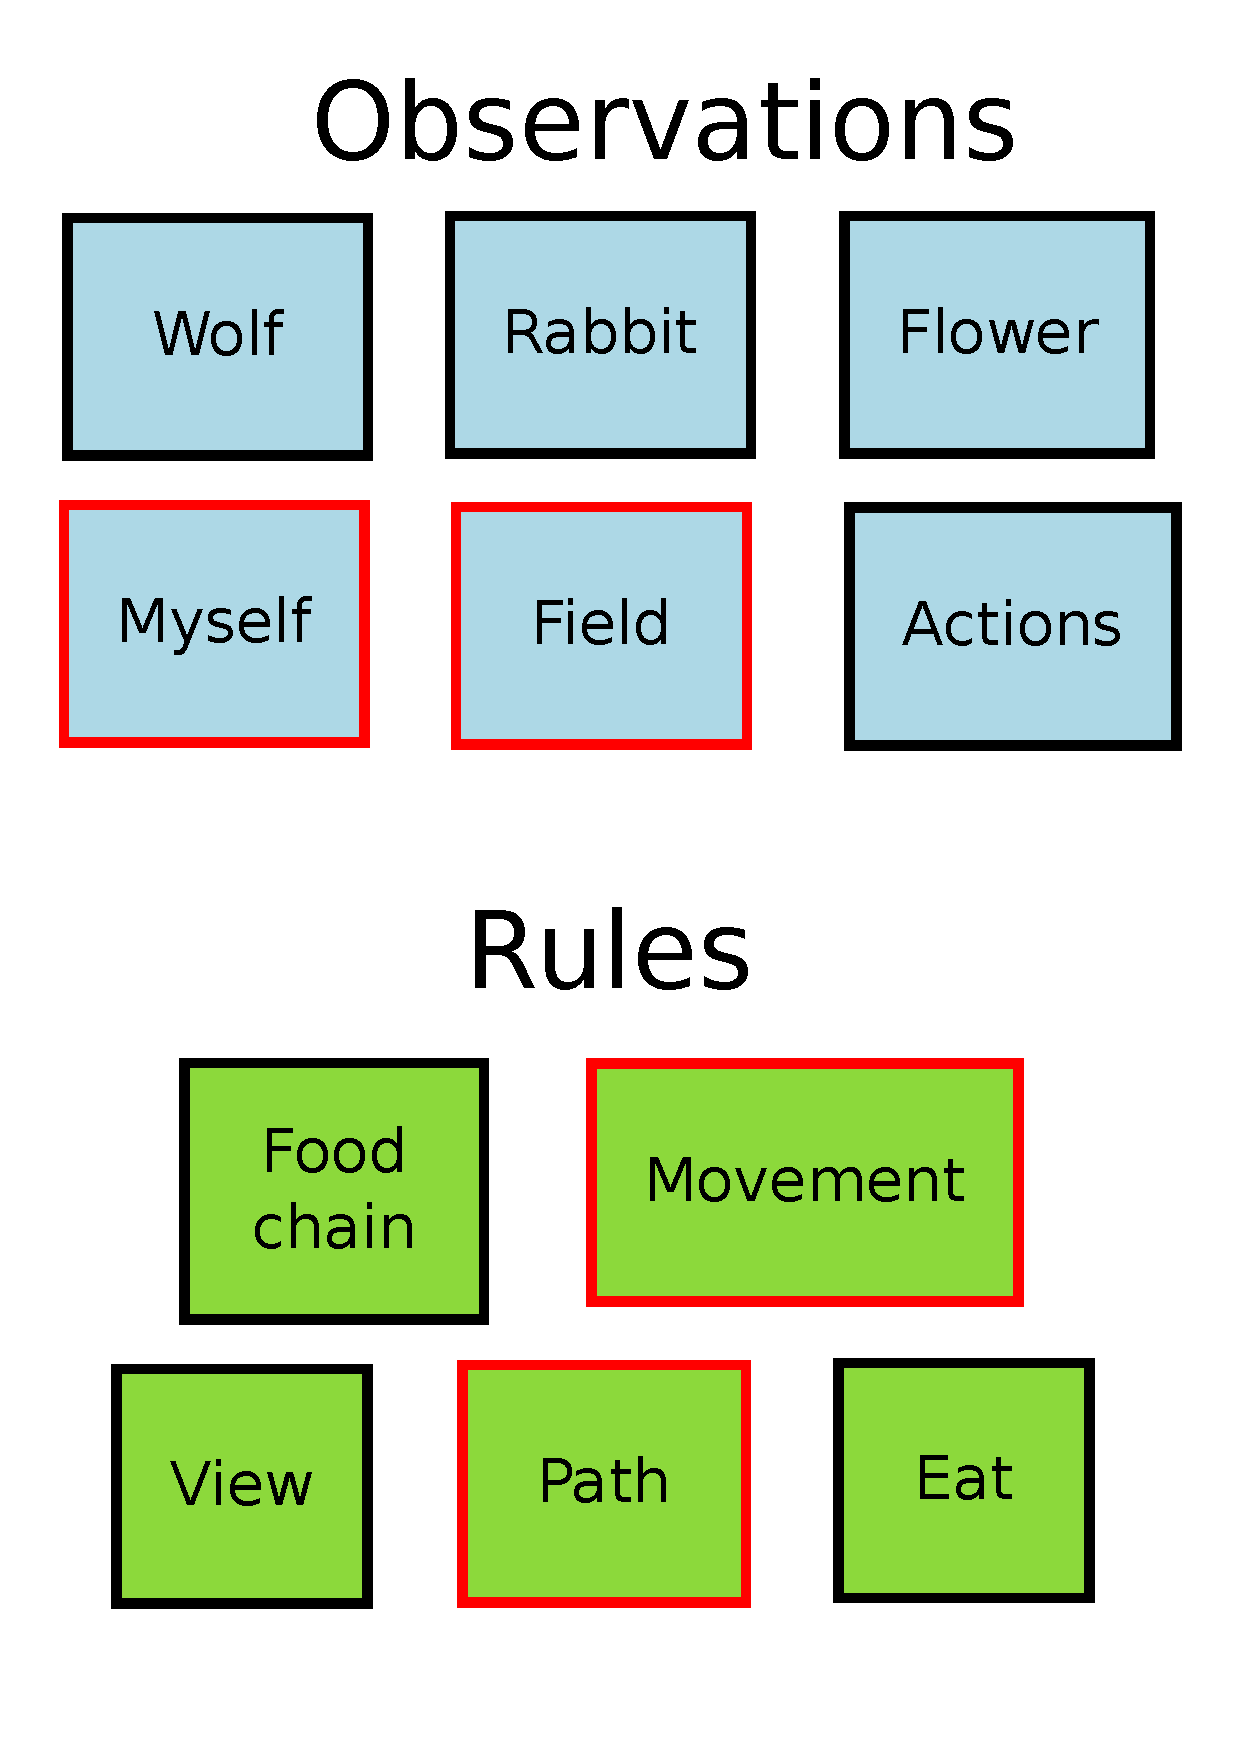
\includegraphics[keepaspectratio=true, scale=0.25]{module_combination.pdf}
		\caption
		{
			\label{module_combination}
			Knowledge base of a wolf, observations modules are blue ones and rules modules are green.
			The module combination \{\textit{Myself}, \textit{Field}, \textit{Movement}, \textit{Path}\} will produce all possible movement of the agent.
		}
	\end{figure}

\subsection{Behaviours}

	In the last section we presented different way to combine rules and observations modules.
	But these combinations are also a kind of knowledge and then can be known by the agent.
	Its a kind of meta-knowledge on our knowledge, more precisely in this case it is knowledge about the use of knowledge.
	This meta-knowledge is a part of the background theory of an agent and could be represented by rules modules.
	But the singularity of this knowledge involve to dedicated a new kind of modules to represent it.

	\begin{definition}[Meta-knowledge module]
		A meta-knowledge module is a set of rules which define the conditions to use an ASP module.
		The content of such module does not change regarding time.
		It contains knowledge on modules combination.	
		The purpose of these modules is to guide reasoning and represent dynamic behaviours.
	\end{definition}
	
	A module combination can represent agent behaviour and by using meta-knowledge modules we can represent it in a elegant way.
	Most simple behaviour can be represented by a simple list of modules to combine, like in example \ref{approach_example} and figure \ref{approach_figure}.
	The module combination \{\textit{Myself}, \textit{Field}, \textit{Rabbit}, \textit{Movement}, \textit{Path}, \textit{Food Chain}, \textit{Eat}\} 
	and \{\textit{Myself}, \textit{Field}, \textit{Wolf}, \textit{Rabbit}, \textit{Movement}, \textit{Path}, \textit{Food Chain}, \textit{View}\} 
	can respectively represent the attack and the approach behaviour of a wolf.
	This two combinations of modules can be known by meta-knowledge modules, in this case theses modules have knowledge on rules and observations modules.
	
	\begin{example}
		\label{approach_example}
		A meta-knowledge module which describe the approach behaviour of wolf:\newline
		\newline
		\textcolor{red}{use\_module}("Myself").\newline
		\textcolor{red}{use\_module}("Wolf").\newline
		\textcolor{red}{use\_module}("Rabbit").\newline
		\textcolor{red}{use\_module}("Field").\newline
		\textcolor{red}{use\_module}("Food chain").\newline
		\textcolor{red}{use\_module}("Path").\newline
		\textcolor{red}{use\_module}("Movement").\newline
		\textcolor{red}{use\_module}("View").
	\end{example}
	
	\begin{figure}
		\centering
		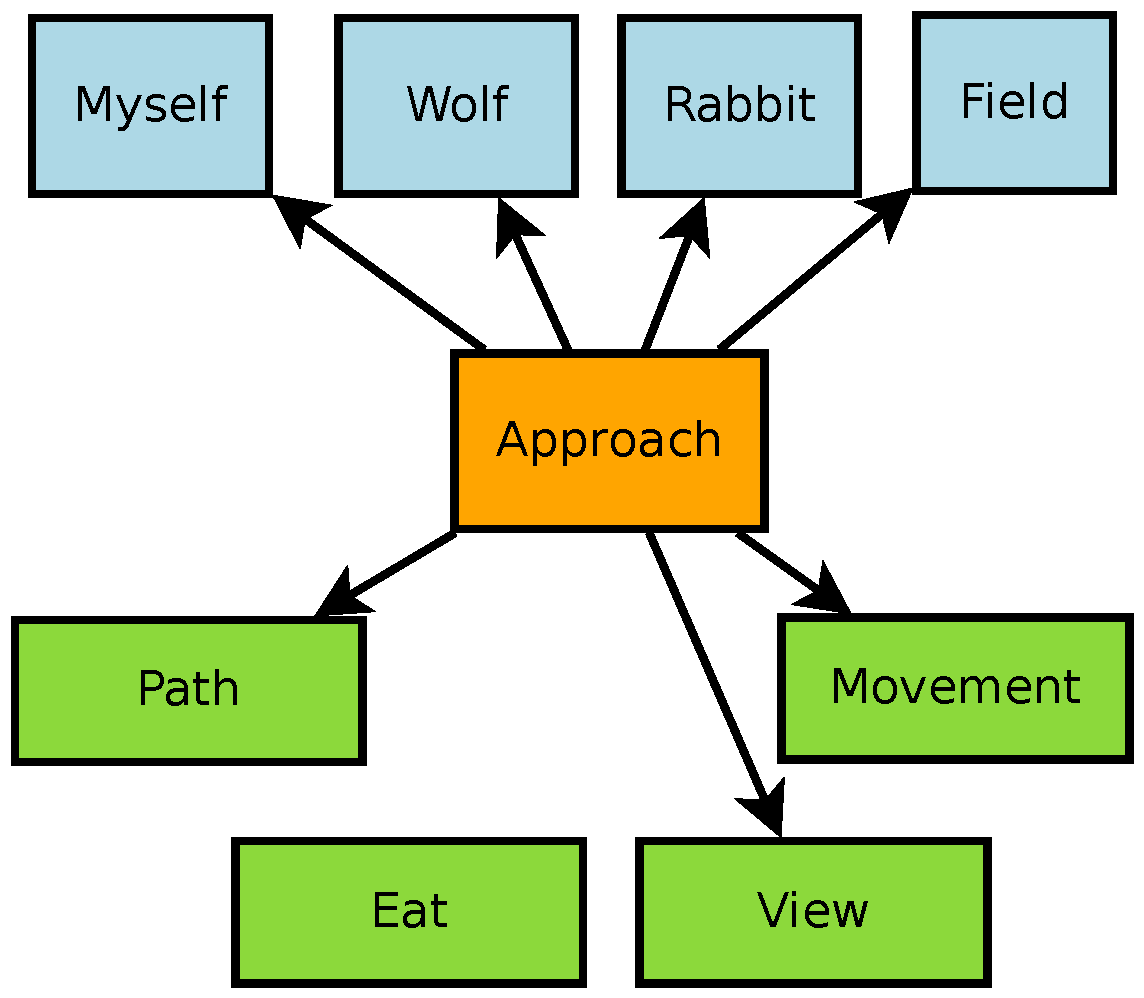
\includegraphics[keepaspectratio=true, scale=0.3]{approach_behaviour.pdf}
		\caption
		{
			\label{approach_figure}
			A meta-knowledge module about approach behaviour, with arrows on modules it knowns.
			Here, \textit{Approach} define the module combination to use to approach a rabbit without being spotted.
		}
	\end{figure}
	
	\begin{example}
		\label{approach_example}
		A meta-knowledge module which describe the attack behaviour of wolf:\newline
		\newline
		\textcolor{red}{use\_module}("Myself").\newline
		\textcolor{red}{use\_module}("Rabbit").\newline
		\textcolor{red}{use\_module}("Field").\newline
		\textcolor{red}{use\_module}("Food chain").\newline
		\textcolor{red}{use\_module}("Path").\newline
		\textcolor{red}{use\_module}("Movement").\newline
		\textcolor{red}{use\_module}("Eat").
	\end{example}
	
	\begin{figure}
		\centering
		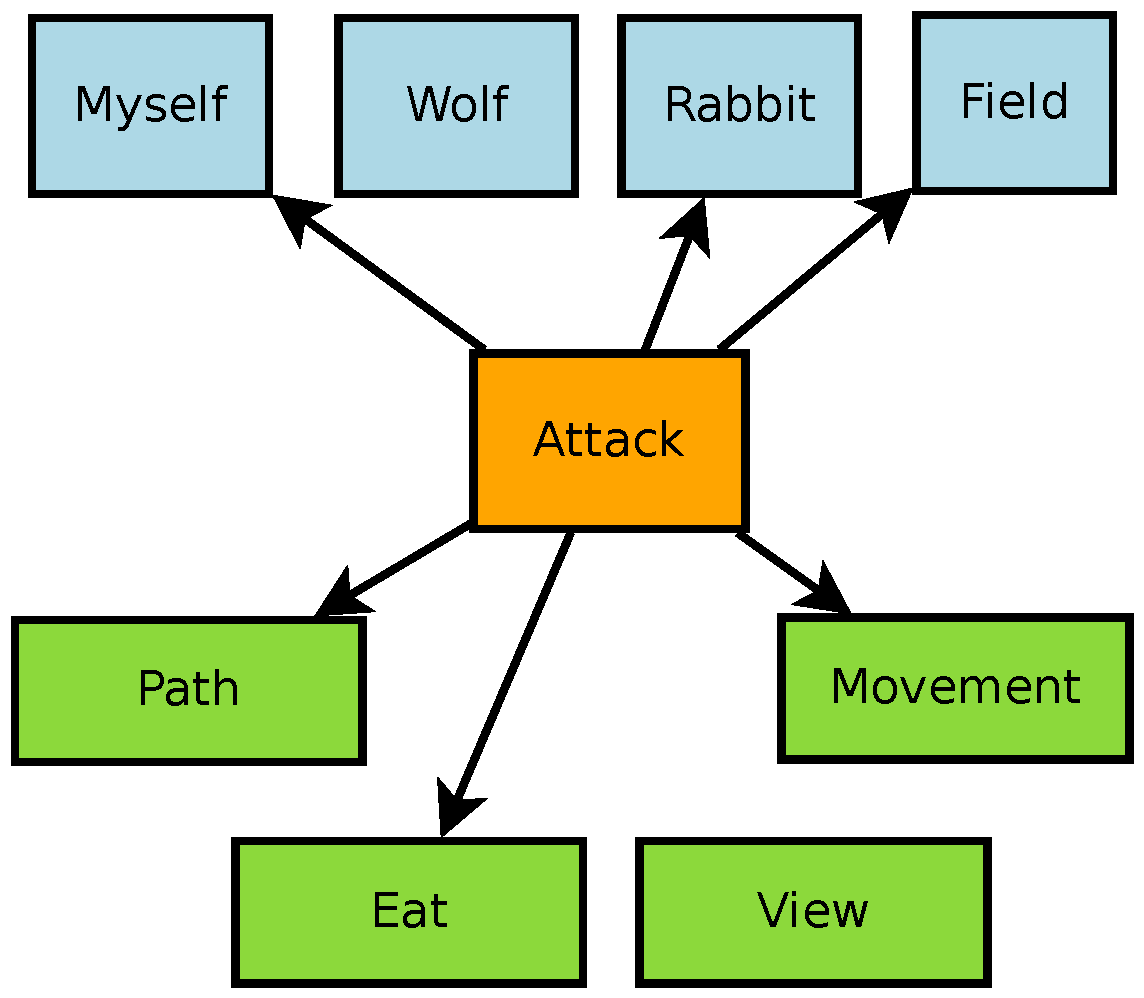
\includegraphics[keepaspectratio=true, scale=0.3]{attack_behaviour.pdf}
		\caption
		{
			\label{approach_figure}
			A meta-knowledge module about attack behaviour.
			Contrary to figure \ref{approach_figure} module \textit{Eat} is use but not \textit{View} and \textit{Wolf}.
			Here, \textit{Attack} define the module combination to use to quickly catch a rabbit.
		}
	\end{figure}
	
	To represent more complex behaviour we can have meta-knowledge modules which have knowledge on other meta-knowledge modules.
	For example we can represent the hunting behaviour of a wolf with such module, like in example \ref{hunting_example} and figure \ref{hunting_figure}.
	If a wolf is spotted it will use the \textit{Attack} module otherwise it will use the \textit{Approach} module.
	Regarding the situation the hunting behaviour will be a sneaky approach or an attack rush.
	Such meta-knowledge modules allows to represent dynamic behaviours which are dependent of the evolution of the environment.
	
	\begin{example}
		\label{hunting_example}
		A meta-knowledge module which describe the hunting behaviour of wolf:\newline
		\newline
		\textcolor{red}{use\_module}("Attack") :- spotted.\newline
		\textcolor{red}{use\_module}("Approach") :- not spotted.\newline
	\end{example}
	
	\begin{figure}
		\centering
		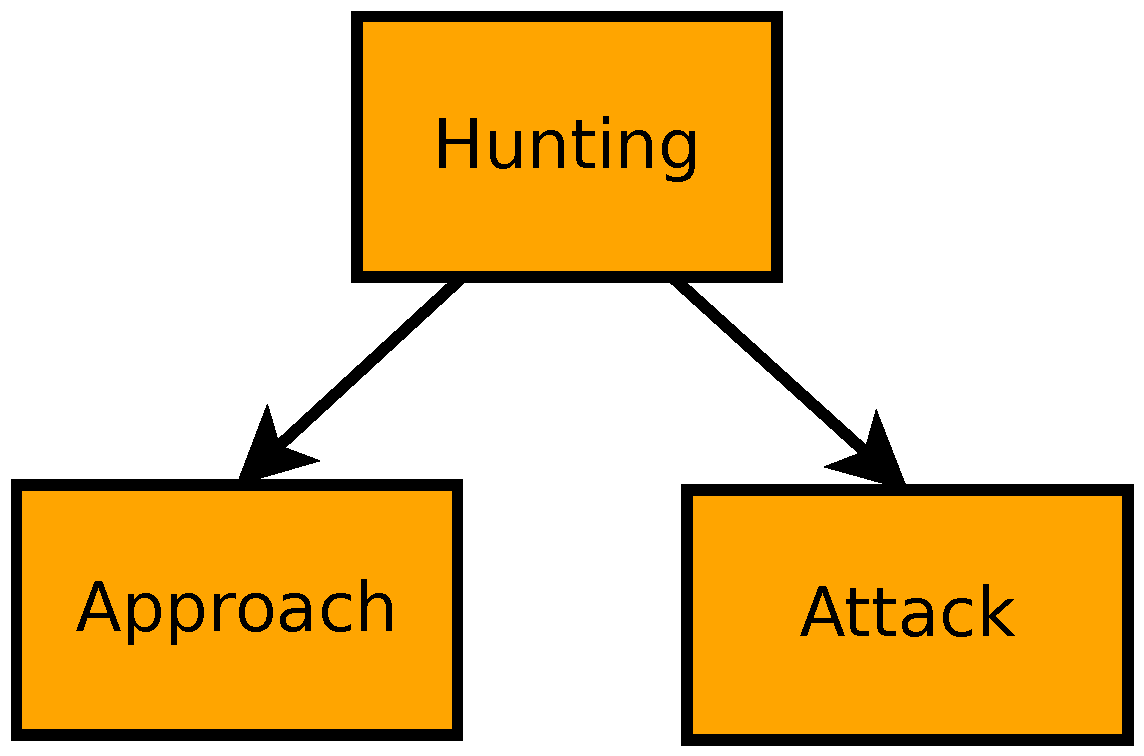
\includegraphics[keepaspectratio=true, scale=0.25]{hunting_behaviour.pdf}
		\caption
		{
			\label{hunting_figure}
			A meta-knowledge module with knowledge about meta-knowledge module.
			Here, regarding the situation the hunting behaviour correspond to a sneaky approach or an attack rush.
		}
	\end{figure}
	
\subsection{Organisation}

	With theses three kind of ASP modules we can now represent agent knowledge and reasoning.
	The figure \ref{organisation_figure} represent the knowledge of a wolf by a graph of modules.
	A node is an ASP module, an edge represent knowledge about modules.
	In this figure, the behaviour of wolf is divide into exploration and hunting.
	The Hunting behaviour is itself divide into approach and attack behaviour.
	We can see here that meta-knowledge modules allows to represent agent behaviours in an elegant and intuitive way.

	\begin{figure}
		\centering
		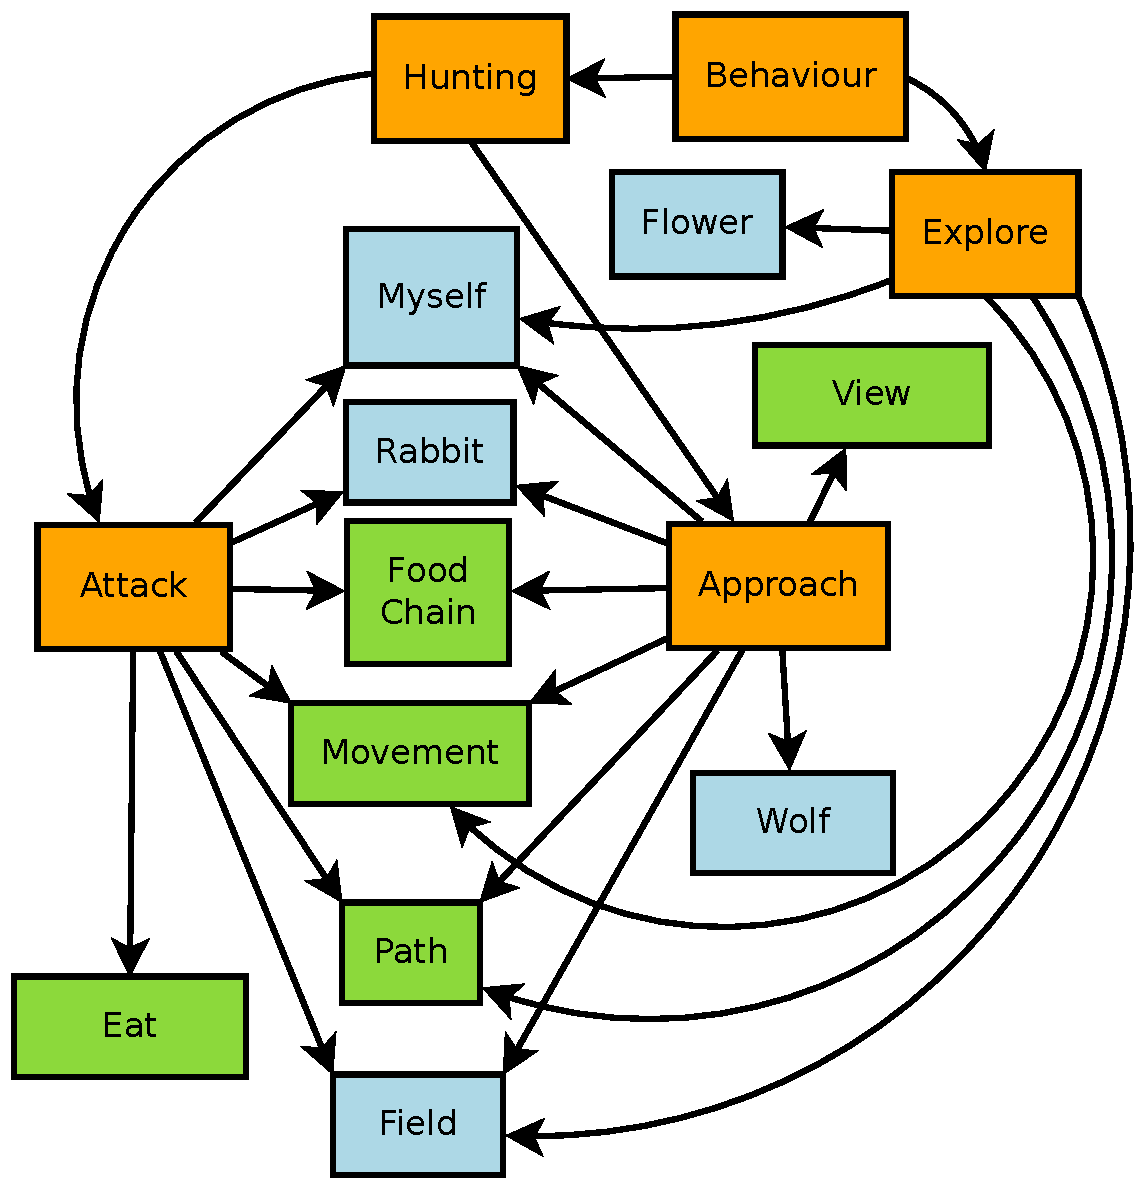
\includegraphics[keepaspectratio=true, scale=0.4]{knowledge_organisation.pdf}
		\caption
		{
			\label{organisation_figure}
			Representation of the knowledge of a wolf by a graph of ASP modules.
		}
	\end{figure}
	
\section{Reasoning}

	In the last section we showed how to represent agent knowledge and behaviours with ASP modules.
	Our design is also dedicated to guide agent reasoning step by step.
	To allow an agent to use our method for reasoning in dynamic environment we implemented a framework.
	Algorithm \ref{framework_algorithm} represent a simplified version of this tool.
	
	Input is a set of modules and output is a set of actions which an agent can perform on its environment.
	It start by compute the combination of input modules and retrieve only one of its answer sets by using the solver \textit{clingo}.
	This answer set is selected randomly from all answer set of the module combination.
	From this answer set we retrieve different commands by extracting keywords.
	By parsing these keyword we extract the combination of modules to use in the next reasoning step and a set of action to perform.
	When the answer set is totally parsed, the cycle restart with the new combination of modules.
	Finally, when there is no more module to combine it return the set of actions to perform.

	Let's take again the example of the figure \ref{organisation_figure} and let's suppose that the wolf just receive a set of new observation from its sensors.
	First our agent will combine theses new observations with the module \textit{Behaviour} to decide if it have to explore the environment or hunt a prey.
	Let's suppose that new observations contains the position of a rabbit, then the next combination of module to use is \{\textit{Hunting}\}.
	Nothing say that the wolf is spotted so the next combination of module to use is \{\textit{Approach}\}.
	Finally the module \textit{Approach} will specify that the last combination of module to use is 
	\{\textit{Myself}, \textit{Field}, \textit{Wolf}, \textit{Rabbit}, \textit{Movement}, \textit{Path}, \textit{Food Chain}, \textit{View}\}.
	The wolf will then perform a movement which allow him to approach the rabbit without being spotted.
	
	In this example we can see that only a part of the knowledge is use for reasoning: 
	modules \textit{Explore}, \textit{Attack}, \textit{Flower} and \textit{Eat} are not used.
	The same knowledge can be represented in only one ASP program, but in this case all knowledge is use.
	Regarding this monolithic representation our method allows to reduce reasoning search space.

	\begin{algorithm}
	\caption{Reasoning}
	\label{framework_algorithm}
	\begin{algorithmic}[1]
	\STATE INPUT : M a set of ASP modules
	\STATE OUTPUT : A a set of actions
	\newline
	\STATE A a set of actions
	\STATE AS an answer set
	\newline
	\STATE A $\leftarrow \emptyset$
	\STATE AS $\leftarrow \emptyset$
	\newline
	\REPEAT
		\STATE // Select \textbf{one} answer set of M
		\STATE AS $\leftarrow$ clingo(M)
		\STATE M $\leftarrow \emptyset$ 
		\newline
		\STATE // Extract framework commands
		\FOR {every literal L of AS}
			\IF {L == "use\_module(Module)"}
				\STATE M $\leftarrow$ M $\cup$ Module
			\ENDIF
			\IF {L == "action(Action)"}
				\STATE A $\leftarrow$ A $\cup$ Action
			\ENDIF
		\ENDFOR
	\UNTIL {M == $\emptyset$} // No more modules to combine
	\newline
	\RETURN A
	\end{algorithmic}
	\end{algorithm}

\section{Experiments}

\section{Conclusions}

	We provide a method based on ASP modules to design agent knowledge.
	This representation allows to intuitively implements dynamic behaviours.
	We also provide a framework which allows agent reasoning via ASP modules.
	Regarding monolithic ASP program, a first improvement of our method is the reduction of reasoning search space.
	Its also cause reduction of code size because modules are reusable for multiple purposes.
	
	In this paper we use ASP but this method can be easily adapted for other programming language, logic or not.
	
%
% The following two commands are all you need in the
% initial runs of your .tex file to
% produce the bibliography for the citations in your paper.
\bibliographystyle{abbrv}
\bibliography{ASP_Modules}  % sigproc.bib is the name of the Bibliography in this case
% You must have a proper ".bib" file
%  and remember to run:
% latex bibtex latex latex
% to resolve all references
%
% ACM needs 'a single self-contained file'!
%

\nocite{*}

\end{document}
